\section{Case Studies}


\subsection{Controlled Studies I - Autoregressive Process} \label{sec:ar-study}


Firstly, the performance of QRAL methodology is evaluated by simulating a widely used autoregressive process and in the sequel estimating the QRAL framework to evaluate if it is capable to recover the parameters fixed at the beginning. 
The aforementioned autoregressive process is set as
\begin{equation}
y_t = \beta_1 y_{t-1} + \varepsilon_t, \quad \varepsilon_t \sim N(0, 1), \label{eq:ar1}
\end{equation}
with length 400 and $\beta_1 = 0.3$. This value was chosen due to the fact that the sample size of RG time series have such length in general.

Three different methods were employed to estimate the process given by (\ref{eq:ar1}):
\begin{enumerate}
\item \textbf{Quantile Regularized Adaptive LASSO (QRAL)}, which estimates one different model for each quantile $Q_{y_t|X}(\alpha,\cdot)$, for all ${j \in J}$. In practice, it means that each coefficient $\beta_{1j}$ is estimated with regularization on each quantile. %As the QRAL estimates a different solution for all every $\alpha$-quantile of $y_t$, the model $$y_t^{\alpha_j} = \beta_{0\alpha_j} + \beta_{\alpha_j} y_{t-1}, \quad \text{for all } j \in J$$ will produce as output a different model for each probability quantile $y_t^{\alpha_j}$.
\item \textbf{Quantile Regression as Koenker (QRK)} as originally proposed by \cite{koenker1978regression}, where each coefficient $\beta_{1j}$ is estimated using QR. 
\item A simple \textbf{Autoregressive (AR)} process.%, the estimated model is $$y_t = \beta_0 + \beta_1 y_{t-1}, j \in J$$. As AR process is not a quantile  One coefficient for  the coefficients $\beta_p(\alpha)$ are all the same, for every quantile (AR(1) estimation).


\end{enumerate}

After simulate 1000 different time series given by Equation (\ref{eq:ar1}), $\beta_{1j}$ was estimated for each one of the aforementioned models. Regarding parameter $\gamma$ (see Eq. (\ref{eq:adalasso-1})-(\ref{eq:adalasso-ult})) it was estimated using CV, as described in section \ref{sec:cv}. Since in this experiment the model has only one lag, model selection will not be evaluated, hence $\lambda=0$.

The main objective of this simulation experiment was to evaluate how our nonparametric methodology can correctly recover the true AR(1) process. The model performance was evaluated by examining how closely the estimated quantiles are from the populational ones. The results for each method are depicted in Figure \ref{fig:boxplot-ar1}, where a boxplot containing the results for the 1000 simulations is shown. %a single boxplot for AR(1) and one for each probability $\alpha$ for QRAL and QRK.
\begin{figure*}[h]
	\centering
	\centerline{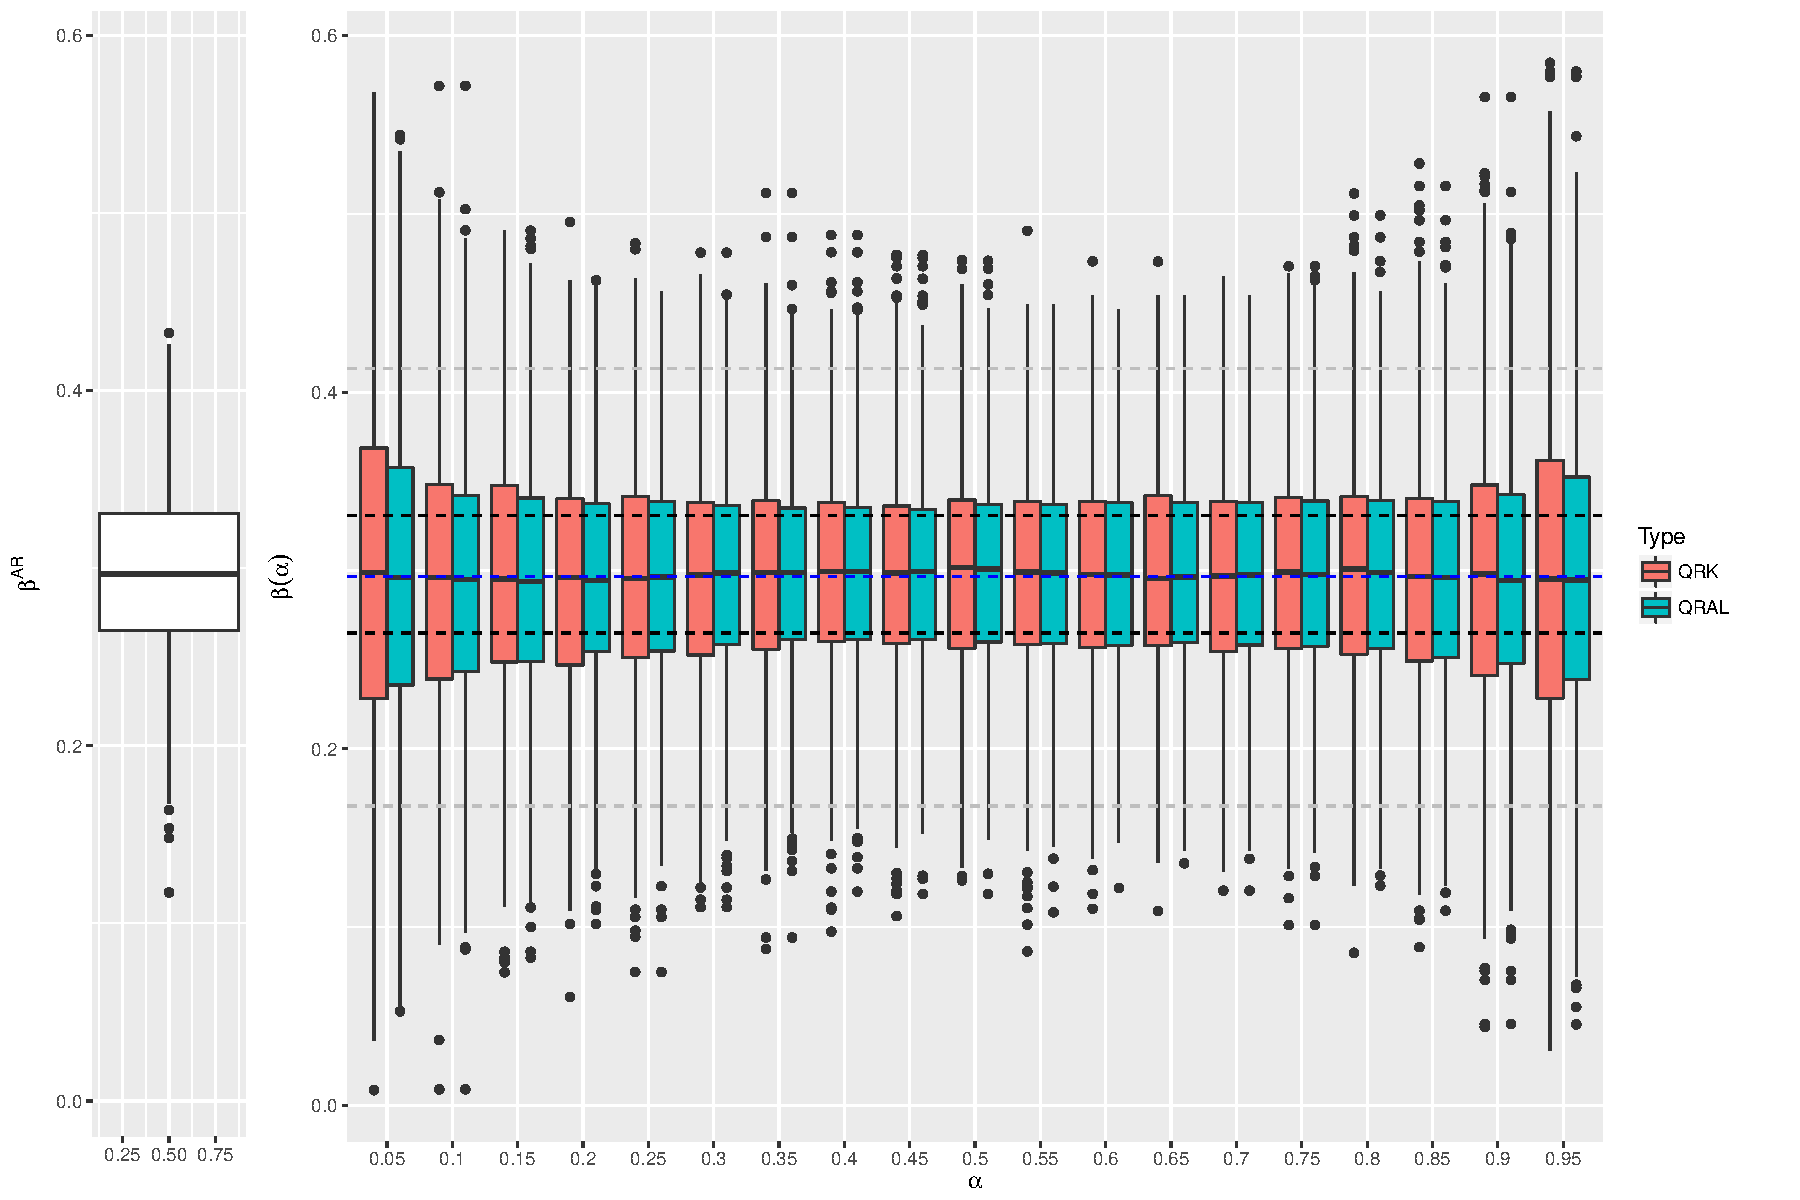
\includegraphics[width=7in]{Images/boxplot-ar1.pdf}}
	\caption{Boxplot showing estimated coefficient after 1000 iterations. On the left hand side, the boxplot of the AR(1) coefficient estimation. Note that for the AR(1) the coefficient is equal for all probabilities $\alpha$. On the right hand side, the boxplot of the regular QR (where $\gamma = 0$) and the QRAL where $\gamma$ is selected using cross-validation. }
	\label{fig:boxplot-ar1}
\end{figure*}
The conclusions from this experiment are: (i) Coefficient estimation errors for the central quantiles are not far from those estimated by the AR; (ii) extreme quantiles are usually harder to estimate, due to having fewer observations; as a consequence, the estimation error increases on the extremes (iii) QRAL has an advantage over QRK in terms of variance of estimators.


\subsection{Controlled Studies II - Quantile Autoregressive Process} \label{sec:qar-study}

In the second controlled study, the performance of the QRAL is evaluated in a Quantile Autoregressive Process. While in the first study the time series $y_t$ is generated by a process with a coefficient $\beta_1$ constant across quantiles, in this experiment $\beta_1$ is a piecewise linear function of $\alpha$, described graphically on Figure \ref{fig:betas-qar}. 
\begin{figure}[h]
	\centering
	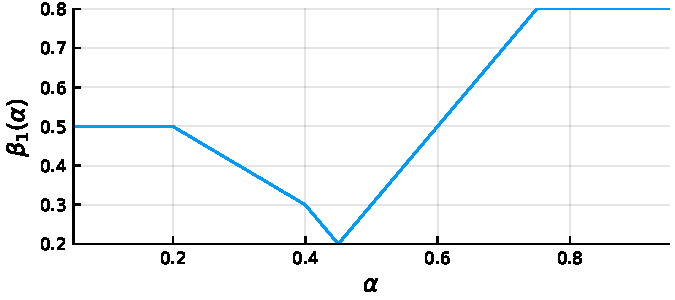
\includegraphics[width=0.8\linewidth]{Images/Betas-Qar.pdf}
	\caption{Coefficient $\beta_1(\alpha)$ of the Autoregressive term $y_{t-1}$ for generating the QAR process.}
	\label{fig:betas-qar}
\end{figure}

The simulation of a QAR process involves two steps. The first is to determine the values of $\beta_0$ from a set of values of $\beta_1(\alpha)$; the latter given as input. These values of $\beta_{0j}$ are the output of the following optimization problem:
\begin{IEEEeqnarray}{lr}
	\underset{\beta_{0}}{\text{min }} \beta_{0,|J|} - \beta_{0,1} \span \\
	\text{subject to} \span \\
	\beta_{0j} + \beta_{j}^T x_{t}  + h \leq \beta_{0,j+1} + \beta_{j+1}^T x_{t}, \span \nonumber  \\
	&\forall t \in T, \forall j \in J_{(-1)},
\end{IEEEeqnarray}
where $h$ is the minimum distance allowed between two neighbour quantiles. If $\beta(\alpha)$ is constant for an interval and $h$ is set to zero, this group of quantiles would superimpose one another. 
Once both vectors $beta_0$ and $\beta_1$ are defined, the 1-step temporal dynamic of the process can be summarized by Figure \ref{fig:qar}. 

\begin{figure}[h]
	\centering
	\centerline{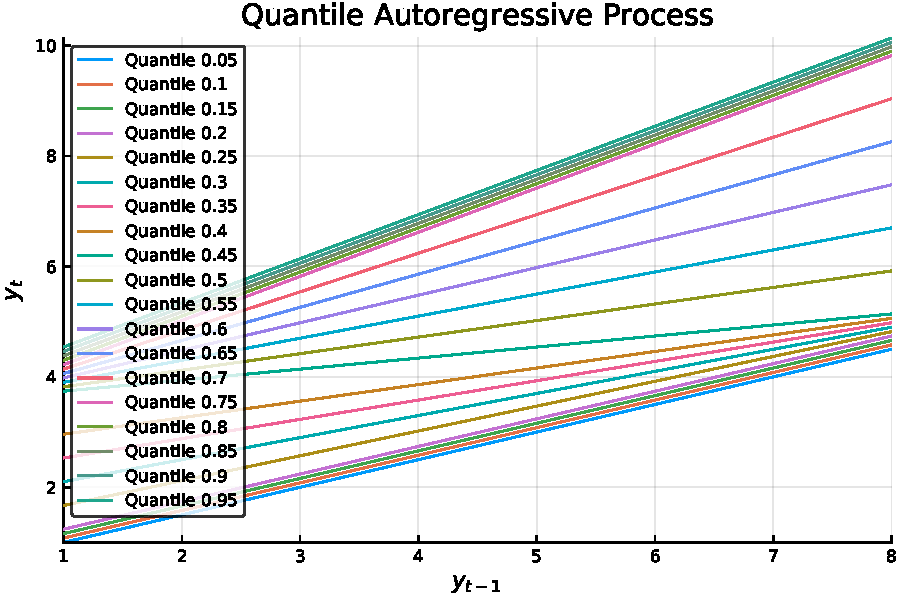
\includegraphics[width=0.8\linewidth]{Images/Qar.pdf}}
	\caption{Quantiles of $y_t$ vs $y_{t-1}$. For each given value of $y_{t-1}$ on the $x$-axis, the curves indicate different levels of quantiles for the values of $y_t$.}
	\label{fig:qar}
\end{figure}

The second step consists in simulating the values of $y_t$. For a given value of $y_{t-1}$, the next term $y_t$ in the time series follows a distribution that can be constructed by the quantiles shown on Figure \ref{fig:qar}. 

This controlled study has the same sample setup as the one in the previous section: 1000 random samples of length 400 and the same three methods tested (QRAL, QRK and AR). The objective of this experiment is to test their performance with respect to their error on the estimation of each coefficient. The summary of results is given by Table \ref{tab:qar-results}, which shows the the aggregated value of quadratic error across all $j \in J$.
The conclusion from this experiment is that both QR methods are much superior than an Autoregressive process such as a AR(1) when the coefficient $\beta$ is allowed to change with probability $\alpha$. 


\begin{table}[h]
\centering
\caption{Cumulated quadratic error of coefficient estimation for each method after 1000 random samples}
\label{tab:qar-results}
\begin{tabular}{lll}
\hline
AR(1) & QR-AdaLASSO & QRK   \\ \hline
38.75 & 5.039       & 5.314
\end{tabular}
\end{table}

\subsection{Real Case Study}

In this section, the QRAL methodology is tested in generating future scenarios of RG. A real time series of Wind Power is the input for estimating coefficients that are employed to generate scenarios by using the procedure described on section \ref{sec:scenario-generation}.
The time series is composed of 31 years (from 1981 to 2011) of monthly observations  of a wind farm located in the Brazilian northeast, measured in Megawatts. The yearly series is shown on Figure \ref{fig:icaraizinho-mensal}.
\begin{figure}[h]
\centering
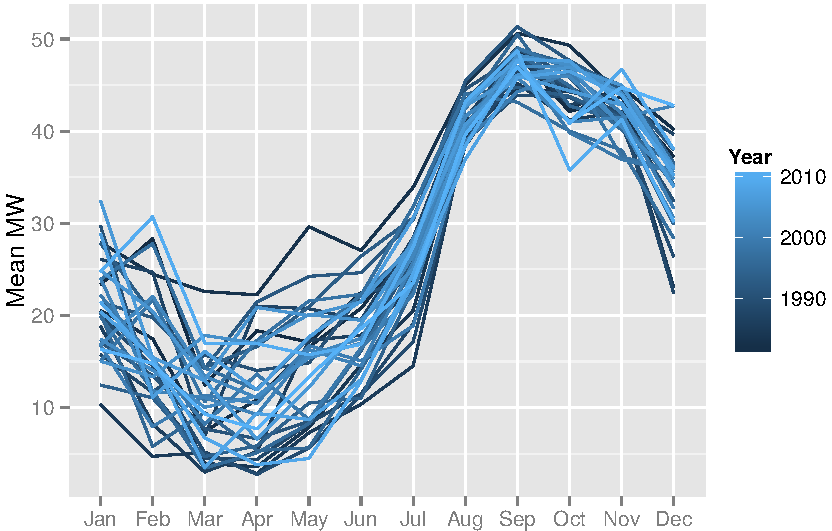
\includegraphics[width=0.8\linewidth]{Images/icaraizinho-mensal2}
\caption{Icaraizinho yearly data. Each serie consists of monthly observations for each year.}
\label{fig:icaraizinho-mensal}
\end{figure}

The last 4 years of this period is leaved as out-of-sample test data. Six different methods are used to generate scenarios: QR-LASSO (Quantile Regularized LASSO), QRAL, QRK, LASSO (original LASSO for QR), AdaLASSO (original AdaLASSO for QR) and SARIMA. The estimated coefficients for the QR based methods are presented on Figure \ref{fig:betas-icaraizinho}. 
\begin{figure*}[h]
	\centering
	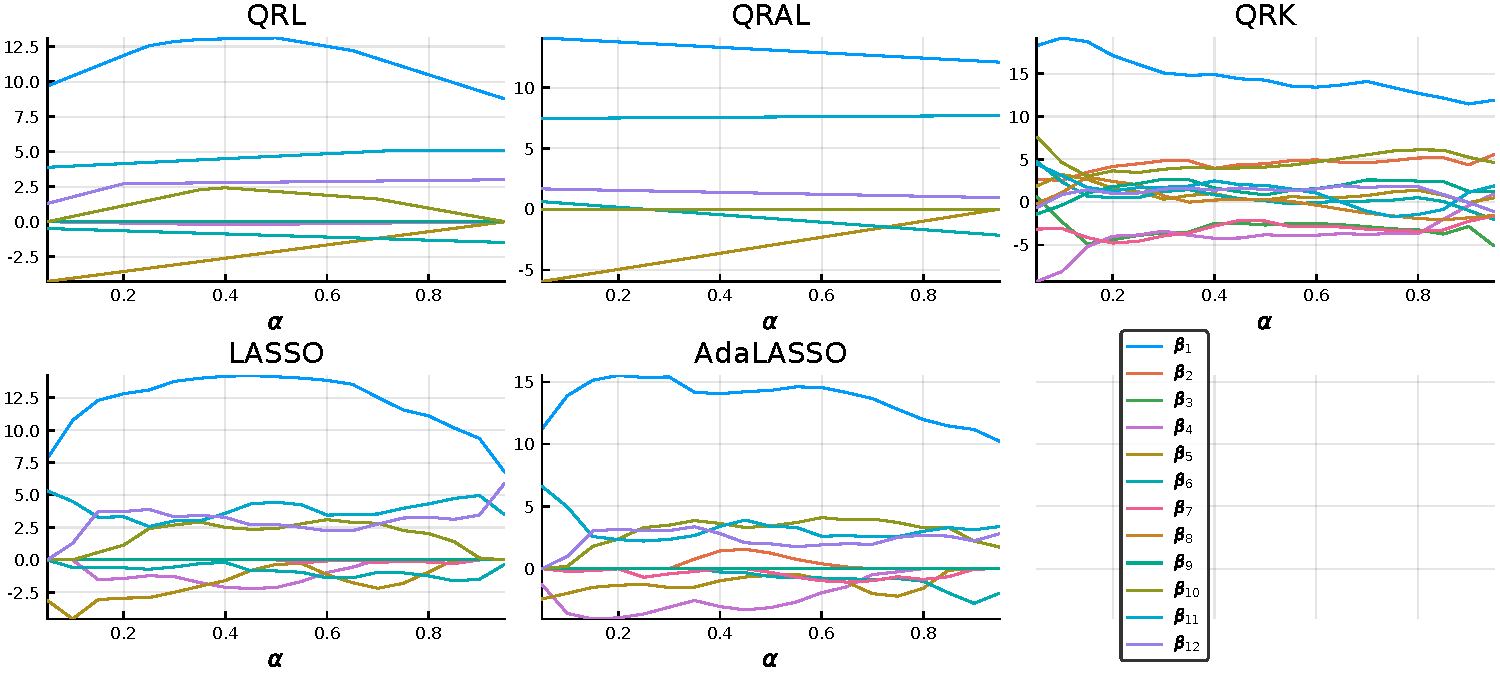
\includegraphics[width=1.0\linewidth]{Images/betas-icaraizinho}
	\caption{Estimated coefficients for each QR based methods. Each line represents the coefficient function $\beta_{p}$ for a given covariate $y_{t-p}$.}
	\label{fig:betas-icaraizinho}
\end{figure*}
The second derivative filter acts reducing the noise, and its effect can be seen clearly when comparing the estimated coefficients of QR-LASSO with the LASSO and the QRAL with the AdaLASSO. 

The accuracy of the generated scenarios - considering the MAPE metric - in recovering the historic quantiles for each month is the metric used for evaluation. These results are shown on Table \ref{tab:results-icaraizinho}. The QRAL is the method that produced the scenarios with the smaller errors.

\begin{table}[h]
\centering
\caption{Cumulated MAPE across all $\alpha_j$ quantiles}
\label{tab:results-icaraizinho}
\begin{tabular}{@{}llllll@{}}
\toprule
QR-LASSO & QR-AdaLASSO & QRK   & LASSO & AdaLASSO & SARIMA \\ \midrule
6.809    & 3.653       & 3.940 & 6.282 & 4.653    & 5.834 
\end{tabular}
\end{table}